%%%%%%%%%%%%%%%%%%%%%%%%%%%%%%%%%%%%%%%%%%%%%%%%%%%%%%%%%%%%%%%%%%%%%%%%%%%%%%%%
% RQ3.tex: Chapter describing the ODE modeling approach to provable guarantees
% of swarm behavior.
%%%%%%%%%%%%%%%%%%%%%%%%%%%%%%%%%%%%%%%%%%%%%%%%%%%%%%%%%%%%%%%%%%%%%%%%%%%%%%%%
\chapter{RQ3: Prediction and Control of SR Systems}%
\label{chap:ode-modeling}
%%%%%%%%%%%%%%%%%%%%%%%%%%%%%%%%%%%%%%%%%%%%%%%%%%%%%%%%%%%%%%%%%%%%%%%%%%%%%%%%
%
\section{Background}\label{ode-modeling:sec:background}
%
To model swarm collective behavior using Ordinary Differential Equations (ODEs),
we consider the individual robot Finite State Machine (FSM) (\cref{fig:fsm});
our FSM is identical to previous work~\cite{Lerman2001,Lerman2002}. Each state
maps directly to a single robot behavior or a set/sequence of robot behaviors
which together make up the robot controller for executing a foraging task. It is
a coarse-grained model of robot behavior, which omits controller details such as
sensing and actuation and contains the \emph{minimum} number of states needed to
describe the system dynamics for the foraging problem.  Such an approach is
generally more mathematically tractable, and if the results of the analysis do
not sufficiently agree with the observed collective behavior, additional states
can be added (see~\cite{Lerman2002} for examples of model refinement by adding
states).
%
\begin{figure}[ht]
  \centering
  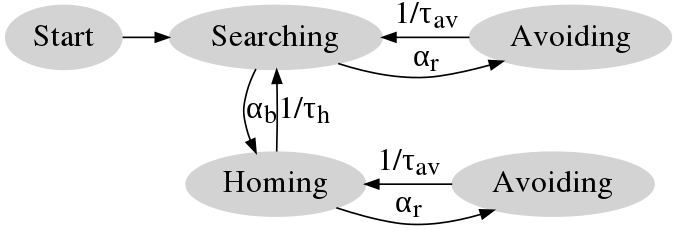
\includegraphics[width=\linewidth]{figures/chapter3/crw-fsm.png}
  \caption{\label{fig:fsm} \footnotesize{State diagram for a single robot. The
      \emph{Avoiding} state is duplicated to uniquely identify the collision
      avoidance context: avoidance while \emph{Homing} or avoidance while
      \emph{Searching}. Transition rates are described
      in~\cref{tab:ode-terms}. Note that the inverse of the amount of time a
      robot spends in a given state (e.g., $\tau_{h}$ for \emph{Homing}) is the
      rate of robots leaving the state. Low level details such as sensing and
      actuation omitted.}}
\end{figure}

% [JRH] Address ijcai#63 comment about the method to go from FSM->ODE
% being case-specific.

Another benefit of the ODE modeling approach is that each of the states
in~\cref{fig:fsm} maps directly to an ODE describing this change, with the
transition rates for states become the ODE terms, and all ODEs can therefore be
directly written down from robot control algorithm characteristics.  We refer
the reader to~\cite{Lerman2001,VanKampen2007} for the theoretical underpinnings
of the validity of this translation, which can be applied to any SR system, not
just those engaged in a foraging task. The quantities modeled in~\cref{fig:fsm}
are listed in~\cref{tab:ode-terms}, and the ODE model of these quantities from
previous work~\cite{Lerman2001,Lerman2002} is summarized
in~\cref{eqn:lerman-ode-searching,eqn:lerman-ode-homing,eqn:lerman-ode-avoiding,eqn:lerman-ode-blocks}.
In our model, shown later in Section~\ref{ssec:method-ode}, we simplify the
original equations and replace some parameters with mathematical derivations.
%
\begin{table}[ht]
  \centering
  \begin{tabularx}{\linewidth}{ p{0.9cm} X }\hline
    {Quantity} &  {Description}  \\
    \hline
    $\alpha_r$ &   {Robot encounter rate of robots \emph{anywhere} in the arena} \\ [1ex]
    $\alpha_{r'}$\string^ & Robot encounter rate \emph{near} the nest \\[1ex]
    $\alpha_r$\string^ &   {Robot encounter rate of robots \emph{far away} from the nest} \\ [1ex]
    $\alpha_b$ &   {Robot encounter rate of blocks} \\ [1ex]
    $\tau_h$ &   {Mean robot homing time} \\ [1ex]
    $\tau_{av}$ &   {Mean robot time spent avoiding collision, per occurrence} \\ [1ex]
    $\SwarmNHoming$ & Mean number of robots returning to nest with blocks \\[1ex]
    $\SwarmNSearching$ & Mean number of robots searching for blocks\\[1ex]
    $\SwarmNAvoidingWhileHoming$ & Mean number of robots avoiding collision while homing\\ [1ex]
    $\SwarmNAvoidingWhileSearching$ & Mean number of robots avoiding collision while searching\\ [1ex]
    $\NBlocksInEnv{t}$\string^ & Mean number of blocks in the arena\\[1ex]
    $\SubAreaNBlocks{t}$* & Mean number of blocks in area $j$ of the arena\\[1ex]
    \hline
  \end{tabularx}\phdcaption{Summary of ODE model components.}{\label{tab:ode-terms}\footnotesize{The component with a * is
      only in our model; components with a \string^ are only in previous work.}}
\end{table}
%
\begin{flalign}
  \frac{d\SwarmNSearching}{dt}
  =~&-\alpha_b\SwarmNSearching\big[\NBlocksInEnv{t} - \SwarmNHoming -\SwarmNAvoidingWhileHoming\big] \label{eqn:lerman-ode-searching} \\
  &-  \nonumber \alpha_r\SwarmNSearching\big[\SwarmNSearching + \TheSwarmSize\big]\\
  &+ \nonumber \frac{1}{\tau_h}\SwarmNHoming + \frac{1}{\tau_{av}}\SwarmNAvoidingWhileSearching
\end{flalign}
%
% [JRH] Add more explanation for ODE terms in original model to address IJCAI
% reviewer#7 comment.
\cref{eqn:lerman-ode-searching} describes the change in the number of robots in
the searching state. It decreases as searching robots pickup blocks or encounter
other robots and switch to collision avoidance. The rate at which robots leave
the searching state and switch to collision avoidance,
$\alpha_{r}\SwarmNSearching[\SwarmNSearching + \TheSwarmSize]$, can be
understood as follows. When a searching robot encounters another searching
robot, both switch to the collision avoidance state, decreasing the
$\SwarmNSearching$ by two; when a searching robot encounters either a homing
robot or a robot already in the collision avoidance state, $\SwarmNSearching$
decreases by one. The total decrease is then proportional to
$2\SwarmNSearching + \SwarmNHoming + \SwarmNAvoidingWhileSearching +
\SwarmNAvoidingWhileHoming = \SwarmNSearching + \TheSwarmSize$. Finally,
searching robots encounter other robots at rate $\alpha_r$, regardless of what
state the other robot is in.~\cref{eqn:lerman-ode-searching} increases as homing
robots deposit blocks in the nest or as searching robots exit the collision
avoidance state.
%
\begin{flalign}
  \frac{d\SwarmNHoming}{dt} =~&
  \alpha_b\SwarmNSearching\big[\NBlocksInEnv{t} - \SwarmNHoming -\SwarmNAvoidingWhileHoming\big] \label{eqn:lerman-ode-homing} \\
  &- \nonumber \alpha_{r'}\SwarmNHoming\big[\SwarmNHoming + \TheSwarmSize\big]\\
  & \nonumber  - \frac{1}{\tau_h}\SwarmNHoming + \frac{1}{\tau_{av}}\SwarmNAvoidingWhileHoming
\end{flalign}
%
\cref{eqn:lerman-ode-homing} describes the change in the number of robots in the
homing state. It increases as robots acquire and pickup blocks or leave the
collision avoidance state. The term \linebreak
$\alpha_{r'}\SwarmNSearching[\SwarmNHoming + \TheSwarmSize]$ can be understood
similar to the one in~\cref{eqn:lerman-ode-searching}. The model makes the
assumption that the rate at which homing robots encounter other robots is
different than for searching robots, reasoning that there will be more
congestion near the nest, and therefore uses a separate parameter $\alpha_{r'}$
to account for this. \cref{eqn:lerman-ode-homing} decreases as robots enter the
collision avoidance state or deposit their block in the nest.

\begin{flalign}
  \frac{d\SwarmNAvoidingWhileSearching}{dt} =~& \alpha_{r'}\SwarmNHoming\big[\SwarmNHoming +
  \TheSwarmSize\big] - \frac{1}{\tau_{av}}\SwarmNAvoidingWhileSearching \label{eqn:lerman-ode-avoiding}
\end{flalign}
%
\cref{eqn:lerman-ode-avoiding} describes the change in the number of
robots avoiding collision with other robots.
%
\begin{flalign}
  \frac{d\NBlocksInEnv{t}}{dt} =~&-\frac{1}{\tau_h}\SwarmNHoming\label{eqn:lerman-ode-blocks}
\end{flalign}
%
\cref{eqn:lerman-ode-blocks}
describes the change in the number of free blocks available for robots to find;
it decreases whenever a searching robot acquires a block (i.e., once deposited
in the nest, blocks are not re-distributed in the arena).

\section{Related Work}\label{ode-modeling:sec:rw}
%
A promising mathematically rigorous methodology utilizing macro- and microscopic
models for group dynamics and individual behavior over
% [JRH] Thesis:
% ~\cite{Dorigo2014,Lerman2002,Berman2007,Galstyan2005,Sugawara1997}
time has been developed~\cite{Lerman2002,Berman2007,Galstyan2005,Sugawara1997},
which sidesteps the difficulty in modeling the average behavior of the swarm,
instead models the \emph{change} in the average swarm behavior, which is much
easier.  It uses (1) differential equations to model the behavior of the
\emph{average} number of robots in $\TheSwarm$ in a given state, (2) discrete
difference equations to model the stochastic transitions between robot states,
and (3) stochastic simulation of discrete difference equations to compute state
transition rates for all robots. It draws on implementations of the stochastic
master equation in chemistry and statistical
physics~\cite{VanKampen2007}. Through the usage of rate constants and population
fractions in each state, it is possible to mathematically assess the general
behavior of a system under a variety of stochastic circumstances. Most
importantly, this approach has predictive control and performance
guarantees---crucial components to translating laboratory models into viable
real-world solutions without needing behavioral characterization of robot swarms
via simulation experiments.

Models in this differential equation paradigm operate on both the forward
problem, i.e., predicting collective behavior from features of the control
algorithm each robot runs~\cite{Lerman2002}, and the inverse problem, i.e.,
incorporating design constraints into algorithm design in order to produce a
desired collective behavior~\cite{Berman2007,Hsieh2008}. However, models are not
overly robust, for two reasons. First, they make large simplifying assumptions
such as homogeneous agent distributions, homogeneous environments (e.g., no
obstacles and/or a completely visible arena), and Markov/semi-Markov
scenarios~\cite{Berman2007}.  Second, they require many free parameters and
extensive post-hoc model fitting which are specific to the implementation of the
algorithm under study. Nevertheless, many notable applications of various
flavors of this methodology have appeared in the literature, demonstrating its
practical utility. A few noteworthy examples include the stick pulling
experiment~\cite{Ijspeert2001}, foraging of green/red pucks using agent
memory~\cite{Lerman2003a}, the ``house hunting
model''~\cite{Hsieh2008,Berman2007}, and ant-inspired models that collaborate
with or without communication~\cite{Sugawara1998,Sugawara1997}.

%%% Local Variables:
%%% mode: latex
%%% TeX-master: "../thesis"
%%% End:
